% This is "aamas2012 .tex" August 2012 
% This file should be compiled with "aamas2012 .cls" 
% This example file demonstrates the use of the 'aamas2012 .cls'
% LaTeX2e document class file. It is for those submitting
% articles to AAMAS 2012  conference. This file is based on
% the sig-alternate.tex example file.
% The 'sig-alternate.cls' file of ACM will produce a similar-looking,
% albeit, 'tighter' paper resulting in, invariably, fewer pages.
% than the original style ACM style.
%
% ----------------------------------------------------------------------------------------------------------------
% This .tex file (and associated .cls ) produces:
%       1) The Permission Statement
%       2) The Conference (location) Info information
%       3) The Copyright Line with AAMAS data
%       4) NO page numbers
%
% as against the acm_proc_article-sp.cls file which
% DOES NOT produce 1) thru' 3) above.
%
% Using 'aamas2012 .cls' you don't have control
% from within the source .tex file, over both the CopyrightYear
% (defaulted to 200X) and the IFAAMAS Copyright Data
% (defaulted to X-XXXXX-XX-X/XX/XX).
% These information will be overwritten by fixed AAMAS 2012  information
% in the style files - it is NOT as you are used with ACM style files.
%
% ---------------------------------------------------------------------------------------------------------------
% This .tex source is an example which *does* use
% the .bib file (from which the .bbl file % is produced).
% REMEMBER HOWEVER: After having produced the .bbl file,
% and prior to final submission, you *NEED* to 'insert'
% your .bbl file into your source .tex file so as to provide
% ONE 'self-contained' source file.
%

% This is the document class for full camera ready papers and extended abstracts repsectively 

\documentclass{aamas2012}
\usepackage{amsfonts} % if you want blackboard bold symbols e.g. for real numbers
\usepackage{graphicx} % if you want to include jpeg or pdf pictures
\usepackage{lmodern}
\usepackage{amsmath}
\usepackage{amssymb}
\usepackage{algorithmic}
\usepackage{algorithm}


\usepackage{pgfplots}
\usepackage{filecontents}
\pgfplotsset{compat=newest}



\begin{filecontents}{testdata2.dat}
x whiskerbottom boxbottom median boxtop whiskertop 
1	 149	 4690	 8019	 10907	 142503
2	 105	 1769	 3017	 3807	 58616
3	 98	 141	 317	 544	 82674
4	 111	 17107	 27189	 46238	 403068
5	 145	 3626	 4461	 6126	 119222
6	 63	 463	 707	 913	 44684
7	 64	 3639	 4707	 7416	 189636
\end{filecontents}

\begin{filecontents}{testdata3.dat}
x whiskerbottom boxbottom median boxtop whiskertop 
1 	2329 	4472 	7075 	11553 	78186
2 	469 	2014 	2626 	3623 	49390
3 	78 	143 	378 	428 	42615
4 	382 	10019 	14027 	24771 	189689
5 	1052 	1116 	1218 	1430 	49089
6 	122 	566 	595	643 	30414
7 	153 	1963 	2585 	3596 	67910
\end{filecontents}

\pgfplotsset{
    box plot/.style={
        /pgfplots/.cd,
        black,
        only marks,
        mark=-,
        mark size=\pgfkeysvalueof{/pgfplots/box plot width},
        /pgfplots/error bars/y dir=plus,
        /pgfplots/error bars/y explicit,
        /pgfplots/table/x index=\pgfkeysvalueof{/pgfplots/box plot x index},
    },
    box plot box/.style={
        /pgfplots/error bars/draw error bar/.code 2 args={%
            \draw  ##1 -- ++(\pgfkeysvalueof{/pgfplots/box plot width},0pt) |- ##2 -- ++(-\pgfkeysvalueof{/pgfplots/box plot width},0pt) |- ##1 -- cycle;
        },
        /pgfplots/table/.cd,
        y index=\pgfkeysvalueof{/pgfplots/box plot box top index},
        y error expr={
            \thisrowno{\pgfkeysvalueof{/pgfplots/box plot box bottom index}}
            - \thisrowno{\pgfkeysvalueof{/pgfplots/box plot box top index}}
        },
        /pgfplots/box plot
    },
    box plot top whisker/.style={
        /pgfplots/error bars/draw error bar/.code 2 args={%
            \pgfkeysgetvalue{/pgfplots/error bars/error mark}%
            {\pgfplotserrorbarsmark}%
            \pgfkeysgetvalue{/pgfplots/error bars/error mark options}%
            {\pgfplotserrorbarsmarkopts}%
            \path ##1 -- ##2;
        },
        /pgfplots/table/.cd,
        y index=\pgfkeysvalueof{/pgfplots/box plot whisker top index},
        y error expr={
            \thisrowno{\pgfkeysvalueof{/pgfplots/box plot box top index}}
            - \thisrowno{\pgfkeysvalueof{/pgfplots/box plot whisker top index}}
        },
        /pgfplots/box plot
    },
    box plot bottom whisker/.style={
        /pgfplots/error bars/draw error bar/.code 2 args={%
            \pgfkeysgetvalue{/pgfplots/error bars/error mark}%
            {\pgfplotserrorbarsmark}%
            \pgfkeysgetvalue{/pgfplots/error bars/error mark options}%
            {\pgfplotserrorbarsmarkopts}%
            \path ##1 -- ##2;
        },
        /pgfplots/table/.cd,
        y index=\pgfkeysvalueof{/pgfplots/box plot whisker bottom index},
        y error expr={
            \thisrowno{\pgfkeysvalueof{/pgfplots/box plot box bottom index}}
            - \thisrowno{\pgfkeysvalueof{/pgfplots/box plot whisker bottom index}}
        },
        /pgfplots/box plot
    },
    box plot median/.style={
        /pgfplots/box plot,
        /pgfplots/table/y index=\pgfkeysvalueof{/pgfplots/box plot median index}
    },
    box plot width/.initial=1em,
    box plot x index/.initial=0,
    box plot median index/.initial=1,
    box plot box top index/.initial=2,
    box plot box bottom index/.initial=3,
    box plot whisker top index/.initial=4,
    box plot whisker bottom index/.initial=5,
}

\newcommand{\boxplot}[2][]{
    \addplot [box plot median,#1] table {#2};
    \addplot [forget plot, box plot box,#1] table {#2};
    \addplot [forget plot, box plot top whisker,#1] table {#2};
    \addplot [forget plot, box plot bottom whisker,#1] table {#2};
}


% if you are using PDF LaTex and you cannot find a way for producing
% letter, the following explicit settings may help
 
\pdfpagewidth=8.5truein
\pdfpageheight=11truein

\begin{document}

% In the original styles from ACM, you would have needed to
% add meta-info here. This is not necessary for AAMAS 2012  as
% the complete copyright information is generated by the cls-files.


\title{AAMAS 2012  Submission in LaTeX Format\titlenote{For use with aamas2012 .cls}}

% AUTHORS


% For initial submission, do not give author names, but the
% tracking number, instead, as the review process is blind.

% You need the command \numberofauthors to handle the 'placement
% and alignment' of the authors beneath the title.
%
% For aesthetic reasons, we recommend 'three authors at a time'
% i.e. three 'name/affiliation blocks' be placed beneath the title.
%
% NOTE: You are NOT restricted in how many 'rows' of
% "name/affiliations" may appear. We just ask that you restrict
% the number of 'columns' to three.
%
% Because of the available 'opening page real-estate'
% we ask you to refrain from putting more than six authors
% (two rows with three columns) beneath the article title.
% More than six makes the first-page appear very cluttered indeed.
%
% Use the \alignauthor commands to handle the names
% and affiliations for an 'aesthetic maximum' of six authors.
% Add names, affiliations, addresses for
% the seventh etc. author(s) as the argument for the
% \additionalauthors command.
% These 'additional authors' will be output/set for you
% without further effort on your part as the last section in
% the body of your article BEFORE References or any Appendices.

%\numberofauthors{8} %  in this sample file, there are a *total*
% of EIGHT authors. SIX appear on the 'first-page' (for formatting
% reasons) and the remaining two appear in the \additionalauthors section.
%

\numberofauthors{1}

\author{
% You can go ahead and credit any number of authors here,
% e.g. one 'row of three' or two rows (consisting of one row of three
% and a second row of one, two or three).
%
% The command \alignauthor (no curly braces needed) should
% precede each author name, affiliation/snail-mail address and
% e-mail address. Additionally, tag each line of
% affiliation/address with \affaddr, and tag the
% e-mail address with \email.
% 1st. author
\alignauthor
Paper  XXX
Kim Svensson\titlenote{Something}\\
       \affaddr{University of Southampton}\\
       \affaddr{Southampton SO17 1BJ}\\
       \affaddr{United Kingdom}\\
       \email{ks6g10@ecs.soton.ac.uk}
% 2nd. author
%\alignauthor
%G.K.M. Tobin\titlenote{The secretary disavows any knowledge of this author's actions.}\\
%       \affaddr{Institute for Clarity in Documentation}\\
%       \affaddr{P.O. Box 1212}\\
%       \affaddr{Dublin, Ohio 43017-6221}\\
%       \email{webmaster@marysville-ohio.com}
% 3rd. author
%\alignauthor Lars Th{\o}rv{\"a}ld\titlenote{This author is the one who did all the really hard work.}\\
%       \affaddr{The Th{\o}rv{\"a}ld Group}\\
%       \affaddr{1 Th{\o}rv{\"a}ld Circle}\\
%       \affaddr{Hekla, Iceland}\\
%       \email{larst@affiliation.org}
}

%\and  % use '\and' if you need 'another row' of author names

% 4th. author
%\alignauthor Lawrence P. Leipuner\\
%       \affaddr{Brookhaven Laboratories}\\
%       \affaddr{Brookhaven National Lab}\\
%       \affaddr{P.O. Box 5000}\\
%       \email{lleipuner@researchlabs.org}

% 5th. author
%\alignauthor Sean Fogarty\\
%       \affaddr{NASA Ames Research Center}\\
%       \affaddr{Moffett Field}\\
%       \affaddr{California 94035}\\
%       \email{fogartys@amesres.org}

% 6th. author
%\alignauthor Charles Palmer\\
%       \affaddr{Palmer Research Laboratories}\\
%      \affaddr{8600 Datapoint Drive}\\
%       \affaddr{San Antonio, Texas 78229}\\
%       \email{cpalmer@prl.com}

%\and

%% 7th. author
%\alignauthor Lawrence P. Leipuner\\
%       \affaddr{Brookhaven Laboratories}\\
%       \affaddr{Brookhaven National Lab}\\
%       \affaddr{P.O. Box 5000}\\
%       \email{lleipuner@researchlabs.org}

%% 8th. author
%\alignauthor Sean Fogarty\\
%       \affaddr{NASA Ames Research Center}\\
%       \affaddr{Moffett Field}\\
%       \affaddr{California 94035}\\
%       \email{fogartys@amesres.org}

%% 9th. author
%\alignauthor Charles Palmer\\
%       \affaddr{Palmer Research Laboratories}\\
%       \affaddr{8600 Datapoint Drive}\\
%       \affaddr{San Antonio, Texas 78229}\\
%       \email{cpalmer@prl.com}

%}

%% There's nothing stopping you putting the seventh, eighth, etc.
%% author on the opening page (as the 'third row') but we ask,
%% for aesthetic reasons that you place these 'additional authors'
%% in the \additional authors block, viz.
%\additionalauthors{Additional authors: John Smith (The Th{\o}rv{\"a}ld Group,
%email: {\texttt{jsmith@affiliation.org}}) and Julius P.~Kumquat
%(The Kumquat Consortium, email: {\texttt{jpkumquat@consortium.net}}).}
%\date{30 July 1999}
%% Just remember to make sure that the TOTAL number of authors
%% is the number that will appear on the first page PLUS the
%% number that will appear in the \additionalauthors section.

\maketitle

\begin{abstract}
A parallel algorithm and implementation using the Nvidia Cuda framework of the dynamic programming algorithm, due To Rothkopf et al. in order to solve the combinatorial auction problem and the complete coalition structure formation problem. 
Using a consumer grade Nvidia GTX 660 Ti for computational test, processing and implementation in order
to compare against an sequential version running on a Intel Xeon W3520 with a clockspeed of 2.67GHz. 
Test results show a speedup factor of 40 with 29 agents with an ever increasing divergence between the CPU and GPU algorithm in terms of growth.
Techniques of memory compression, utilizastion of reduntant operation and further optimisations to implement in order to raise performance.
\end{abstract}

% Note that the category section should be completed after reference to the ACM Computing Classification Scheme available at
% http://www.acm.org/about/class/1998/.

%\category{H.4}{Information Systems Applications}{Miscellaneous}

%A category including the fourth, optional field follows...
%\category{D.2.8}{Software Engineering}{Metrics}[complexity measures, performance measures]

%General terms should be selected from the following 16 terms: Algorithms, Management, Measurement, Documentation, Performance, Design, Economics, Reliability, Experimentation, Security, Human Factors, Standardization, Languages, Theory, Legal Aspects, Verification.

%\terms{Delphi theory}

%Keywords are your own choice of terms you would like the paper to be indexed by.

%\keywords{AAMAS proceedings, \LaTeX, text tagging}

\section{Introduction}

\section{Background}

\subsection{Coalition formation}


\subsection{The {\secit DP} Algorithm} %done


The DP algorithm as shown in algorithm \ref{DP} works by producing two output tables, $O$ and $f$, 
where each table have one entry per coalition structure. 
An entry in $f$ represent a value a certain coalition structure is given, 
while $O$ represent which splitting, if any, maximised the coalition structure for the entry in $f$ which it represent.
More elaborated, given all coalitions of agents $C\subseteq A$, for each coalition in $C$, evaluate all
pairwise disjoint subsets here named splittings on their pairwise collective sum against the coalitions
original value. Given one splitting is greater, update the value of the coalition $f(C) := f(C') + f(C\setminus C')$
and assign $O$ on $C$ to represent the new splitting, $O(C) := \{C',C\setminus C'\}$. These steps are first carried out
on all coalition structures with two agents, continuing until $N$ agents. 
This means, given a coalition structure $S$ with cardinality $|S| = n$, then all coalition structures
for the sizes 1,2,...,n-1 have already been evaluated. The dynamic programing algorithm is entierly deterministic meaning
that even if there was only one or two valuations, the algorithm will evaluate all splittings before it reaches a conclusion.
However this algorithm does not work well with an large amount of agents as it grow exponential and have an time complexity of $O(3^n)$.
As described later in section ?? the part of the algorithm that is parallilsed is the max function on line \ref{lst:line:a}
which handles the evaluation of all splittings of a given coalition structure.

\begin{algorithm}
\caption{Dynamic Programming algorithm \label{DP}}
INPUT: $b$: collection of the bids for all coalitions\\*
VARIABLES: $f$: collection holding the maximum value for all coalitions\\*
$O$: collection holding the most beneficial splitting for all coalitions.
\begin{algorithmic}[1]
\STATE\algorithmicfor\ all $x \in A$, \algorithmicdo  $f(\{x\}):= b(\{x\}),O\{x\}:= \{x\}$ \algorithmicendfor
\FOR{$i := 2$ to $n$}
\FOR{all $C \subseteq A: \vert C \vert == i$}
\STATE $f(C) := max\{f(C\backslash C')+f(C'):C'\subseteq C \wedge 1 \leq \vert C' \vert \leq \dfrac{\vert C \vert}{2}\}$ \label{lst:line:a}
\STATE\algorithmicif $f(C) \geq b(C)$ \algorithmicthen\ $O(C) := C^{*}$ \hfill Where $C^{*}$ maximizes right hand side of line~\ref{lst:line:a} \algorithmicendif
\STATE\algorithmicif $f(C) < b(C)$ \algorithmicthen\ $f(C) := b(C)\wedge O(C) := C$ \algorithmicendif
\ENDFOR
\ENDFOR
\STATE Set $CS^* := \{A\}$
\FOR{all $C \in CS^*$} \label{lst:line:redo}
\IF{$O(C) \neq C$}
\STATE Set $CS^* := (CS^*\setminus \{C\})\cup \{O(C),C\setminus O(C)\}$ 
\STATE Goto \ref{lst:line:redo} and start with a new $CS^*$
\ENDIF
\ENDFOR
\RETURN $CS^*$
\end{algorithmic}
\end{algorithm}

The table $O$ may be discarded and not calculated to reduce the memory requirement by half removing instant access to the final splittings.
These final splittings are easily retrived as outlined in algorithm \ref{idpref}. 
Essentialy, all coalitions in $C \in CS^*$ which value in $f$
is not equal to the initial bid in $b$, find the first splitting that is equal to the value in $f$.
The overhead of this is insignificant as it needs to evaluate at most $n -1$ coalitions compared to the exponential
number of evaluations carried out in the previoius steps\cite{eps265062}.

\begin{algorithm}
\caption{Enumeration of the optimal splittings through re-evaluation of small amount of coalitions \label{idpref}}
INPUT: $b:$ array of the initial bids for all coalitions $C \subseteq A$. 
$f:$ the final evaluated values gathered from evaluating splittings.
\begin{algorithmic}[1]
\STATE Set $CS^* := \{A\}$
\FOR{all $C \in CS^*$} \label{lst:line:redo2}
\IF{$f(C) \neq b(C)$}
\STATE find first $C^*$ where $f(C) = f(C\backslash C^*)+f(C^*):C^*\subseteq C \wedge 1 \leq \vert C^* \vert \leq \dfrac{\vert C \vert}{2}$ \label{lst:line:aa}
\STATE Set $CS^* := (CS^*\setminus \{C\})\cup \{C^*,C\setminus C^*\}$
\STATE Goto \ref{lst:line:redo2} and start with a new $CS^*$
\ENDIF
\ENDFOR
\RETURN $CS^*$
\end{algorithmic}
\end{algorithm}



\subsection{The CUDA Architecture} %done
Graphics Processing Units(GPU) from Nvidia and AMD is highly multithreaded, many-core architectures primarily aimed at 
highly parallel image processing and rendering, however it have in the recent years moved towards supporting general purpose computing through 
the OpenCL and Nvidia CUDA framework.
It does so by devoting a larger amount of transitors towards many computational units rather than data caching and advanced 
flow controll more often seen in CPU architectures.
Nvidia describes their general purpose GPU CUDA architecture as a Single Instruction Multiple Threads (SIMT) architecture, 
meaning groups of multiple threads excecute the same instructions concurrently and is proportional to SIMD architectures. 
This enables their GPUs to be highly advantageous when performing data-independant and non-divergent tasks.

To understand this further the grouping of the threads need to be explained and is outlined in figure \ref{fig:reduction}.
A kernel which is a device specific CUDA function that is called by the sequential host code,
will request a specified number of blocks in a grid of blocks.
Each block may to this date consist of up to 1024 threads depending on the compatability of the card, with a maximum
grid size of $2^{31}-1$ blocks subjected to compatability. When run, the blocks will be distributed onto available multiprocessors,
which then independantly schedule the runtime of the block. Note that blocks may be excecuted concurrently or sequential depending on
the current workload and the number of available multiprocessors.
The block is split into smaller units of 32 threads called warps, all threads within the same warp are always scheduled
the same instruction to be run and this is what embodies the SIMT paradigm. 
Therefore, branching threads causing inter-warp divergence means a warp will have inactive threads not excecuting any instructions, 
which may lead to poor efficiency with worst case of sequential performance. Further, warps are scheduled independantly of eachother
meaning possible concurent excecution of warps.

The threads communicate with each other through writes to various types of memory outlined in table \ref{mem}.
There are three types of thread writable memory in the architecture; registers and local memory are each threads
coupled memory which is not volatile and may be shared with other threads inside the same warp as described in section \ref{reduction}. 
Shared memory is as its name tells shared between all threads within the same block, as it may be written to by any thread within the block
it should be treated as volatile, thus syncronization inside the block have to be consider whilts dealing with shared memory.
Finally, global memory is the only persistant memory which will persist between each kernel call, it may be manipulated by the host,
but also by any thread, and is the only means of communication inbetween kernels, blocks, and the host. It to should be considered voaltile.

Regarding access to the global memory, certain access patterns must be followed in order maximise performance. 
For global memory, it is important to note that each load request from memory will fetch in cachelines of size $32*wordsize$,
meaning cachelines of 32, 64, and 128 bytes each when pulling the primitives char, short and int respectively.
The reason for this is the fact mentioned earlier, all 32 threads within the same warp issue the same instruction, 
thus each warp fetches 32 entities of a specific word type.
As a result, if the memory reads within a warp is not coalesced(grouped within the same cacheline) within consecutive words, the effective bandwidth will drop immediately.


\begin{table}
\centering
\caption{Memory scope, lifetime, and speed \label{mem}}
\begin{tabular}{|l|l|l|l|} \hline
Type&Scope&Lifetime&Relative Speed \\ \hline
Register&Thread \& Warp&Thread&Fastest\\
Shared&Block&Block&Fast\\
Global&Kernel \& Host&Program&Slow\\
\hline\end{tabular}
\end{table}

\subsection{Data structure} %done
How the data is represented and structured is important, 
especially in bandwidth bound algorithms where the majority of time
is spent fetching data from memory and the arithmetic overhead is low.
Selecting the right composition will reduce the memory requirements substantialy.
Given the two entities of data that is needed to be represented for each coalition structure, 
the coalition structure itself and its value in $f$. 
Memory constraints will be imposed given a large amount of agents as a result of DP's exponential growth. 
In order to minimize memory usage several technices were used. 
Representing a coalition structures members as an array of values,
where each value represent a distinct agent may seem intinuative at first. 
However, if the members are represented as bits set in a fixed sized integer, the memory
requirement will be reduced substantialy as shown by previoius studies.\cite{boyer2012solving}
If solving for the complete coalition structure formation problem with n agents representing members as an array of values.
There are \begin{math}\dbinom{n}{i}\end{math} coalition structures of size $i$, where
$i$ entries have to be stored per coalition structure.
The total number of values needed to store just to represent the coalition structures is there for equal to:
\begin{displaymath}\sum_{i=i}^{n} \dbinom{n}{i}*i\end{displaymath}

Given the same constraints, representing the coalition structure as an fixed sized integer, it is only 
needed to store one entry per coalition structure, totaling to \begin{math}2^n-1\end{math} data points.

To give an example, with four agents $A = {f_1,f_2,f_3,f_4}$, the coalition $C = {f_1,f_3,f_4}$ would be represented
as $C = 1101$ in the binary system and $11$ in the decimal system. Therefore, if the coalition
structure is represented as an integer it can implicitly be stored as an index 
to its coalition value, by enumerating it on runtime. That means the only
memory constraint on the system is the store all the values for all the coalition structures.

\subsubsection{Coalition Structure Splittings}

\begin{table}
\centering
\caption{Splittings of $C = \{f_1,f_3,f_4\}$ Binary $C = 1101$ \label{split}}
\begin{tabular}{|l|c|c|c|} \hline
Set& $\{f_1\}$\hfill$\{f_3,f_4\}$ &$\{f_3\},\{f_1,f_4\}$&$\{f_4\},\{f_1,f_3\}$ \\ 
system&&& \\ \hline	
Binary&0001\hfill 1010&0010\hfill 1001&1000\hfill 0011 \\
system&&& \\
\hline\end{tabular}
\end{table}

\begin{algorithm}
\caption{initShift input $Coalition:C$ \label{initshift}}
\begin{algorithmic}[1]
\STATE $t :=C$
\STATE $count := 0$
\WHILE{$t > 0$} {
\STATE $index := FindFirstSet(t)$
\STATE $shift_{count} := index$
\STATE $nullBit(t,index)$
\STATE $count++$
}
\ENDWHILE
\RETURN shift
\end{algorithmic}
\end{algorithm}


Splittings as mentioned are pairwise disjoint subsets of a coalition structure, 
given the coalition structure $C = \{f_1,f_3,f_4\}$ the splittings
are shown in table \ref{split}. In order to generate the splitting there is essentially two methods used, 
the, initShift, initialSplit and nextSplit methods. 
The function initShift as detailed in algorithm \ref{initshift} is necessary to setup the environment for 
all calls to initialSplit, what it does is using the bit operation $find first set$ to find the indexes of all bits set
in from the integer coalition input. This will give each entry in the $shift$ array an unique number. 
This unique numbers will be used by initialSplit to distribute the bits of the count to fit the configurations bits.
It does so by taking a count as input representing which n'th splitting should be created, finds the index of its 
set bits, and finaly left shifts each bit with the value in the shift array its index reference to.

nextSplit works through a recurence relation which means in order to have 
concurent threads independant of eachother, an initial splitting for each thread have to be calculated using initialSplit. 
initialSplit works by first genereting an packed index array of which bits are set in the coalition structure using initShift.
Given which n'th splitting it should generate, it distributes the bits of $n$ to the corresponding bits of coalition $C$. 
Thereafter nextSplit will be used to generate the next splitting. 




\begin{algorithm}
\caption{ nextSplit input $Coalition:C$ $Splitting:S$}
\begin{algorithmic}[1]
\STATE $C' := twosComplement(C)$
\STATE $S' := bitwiseAND((C'+S),C)$
\RETURN $S'$
\end{algorithmic}
\end{algorithm}

\begin{algorithm}
\caption{initialSplit input $Count:n, Coalition:C$}
\begin{algorithmic}[1]
\STATE $t := n$
\STATE $S := 0$
\WHILE{$t > 0$} {
\STATE $index := FindFirstSet(t)$
\STATE $S := S + leftShift(1,shift_{index,C})$
\STATE $nullBit(t,index)$??
}
\ENDWHILE
\RETURN $S$
\end{algorithmic}
\end{algorithm}

\begin{algorithm}
\caption{Fetch using Collision detection \label{collision}}
Input:
Index:$\psi$ \hfill Which n'th splitting should be generated
Index:$z$ \hfill The index in $\upsilon$ for the coalition structure that is evaluated 

Variables:Value $\alpha $: \hfill Holds temporary values

\begin{algorithmic}[1]
    \STATE $C_{0} := initialSplit(\psi,CS_0)$ \label{lst:line:startcol}
    \STATE $C_{1} := initialSplit(\psi,CS_1)$
    \STATE $\upsilon_{0,z} := f(C_{0})$ \label{lst:line:fetch}
    
    \IF{$C_{1} = C_{0}$} \label{lst:line:firstif}
      \STATE $\upsilon_{0,z+1} := \upsilon_{0,z}$
      \ELSE
      \STATE $\upsilon_{0,z+1} := f(C_{1})$
     \ENDIF \label{lst:line:firstifend}
    \STATE $C_{0} := CS_0\backslash C_{0}$ \label{lst:line:startend}
    \STATE $\alpha := f(C_{0})$
    \STATE $C_{1} := CS_1\backslash C_{1}$
    \IF{$C_{1} = C_{0}$}
      \STATE $\upsilon_{0,z+1} := \upsilon_{0,z+1}  + \alpha$
    \ELSE
      \STATE $\upsilon_{0,z+1} := \upsilon_{0,z+1} + f(C_{1})$
    \ENDIF
    \STATE $\upsilon_{0,z} := \upsilon_{0,z}  + \alpha$ \label{lst:line:endend}
\RETURN $\upsilon$
\end{algorithmic}
\end{algorithm}

\subsubsection{Collisions between Splittings of Coalitions} \label{sectionsplit}
Given that each thread evaluate several splittings over numerous coalition structures in parallel, 
it is bound that splittings on two coalition structures that overlap will have splittings that collide.
A collision means that splittings of coalition structures contain at least one identical subset shared between them.
\begin{displaymath}\forall S\subset C \wedge S' \subset C' : C \cap C' \neq \emptyset \Rightarrow \exists S \wedge S' : S = S'\end{displaymath}
For all splittings of $C$ and $C'$ where the coalition structures intersect, there must excist at least one splitting shared between them.

The number of splittings that collide is dependant on how many common members the coalitions have in common.
\begin{displaymath}2^{n-1}-1:C\neq C'\wedge |C \cap C'| = n \wedge n > 1 \end{displaymath}
Specifically, the number of splittings incommon is how many splittings
can be done all the members in common.
Normaly, each splitting would be fetched from global memory resulting in it being fetched several times, 
if it have not been evicted from the cache memory.

By using collision detection as described in algorithm \ref{collision} the number of reduntant fetches may be reduced.
It works by evaluating two or more coalitions at the same time, lines \ref{lst:line:startcol} to \ref{lst:line:fetch} generates
the intial splittings and fetches the value for the first splitting. It then trough lines \ref{lst:line:firstif} to \ref{lst:line:firstifend}
checks wheater the splitting of the second splitting is equal to the first. 
If so assign it the first splittings value, else fetch its own value from global memory. 
Finally, the last lines does the same thing as above just that it does that on the pairwise disjoint subset, 
and the first splittings next value is stored in an temporary variable. 
The more splittings that are evaluated at the same time and checked against eachother, the less reduntant memory fetches are done.


\subsubsection{Reduction} \label{reduction} %done
\begin{figure*}
\centering
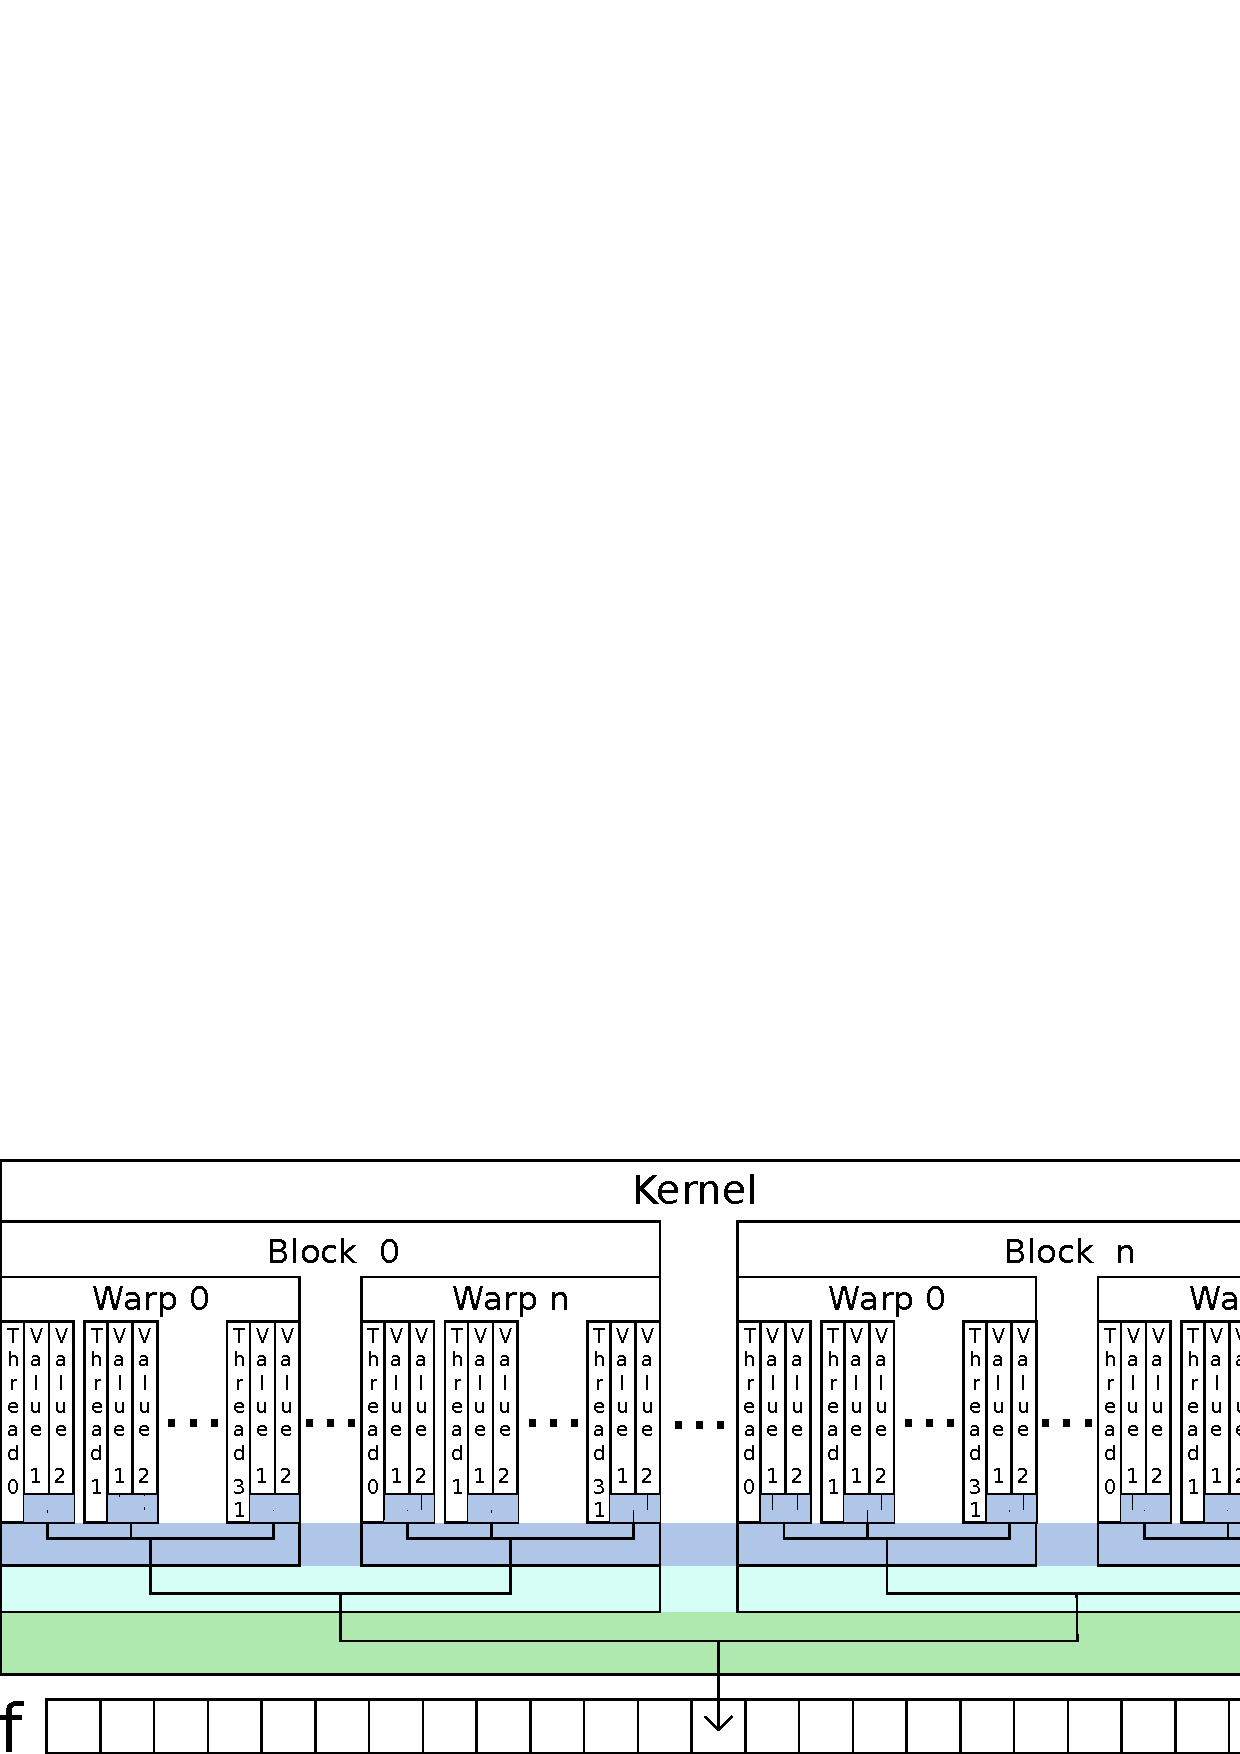
\includegraphics[width=\linewidth]{reduction.png}
\caption{Outline of reduction across thread, warp, block and kernel \label{fig:reduction}}
\end{figure*}

As the evaluation of each coalition structure is to find the splitting 
of the coalition structure which maximises the value of the coalition structure,
it is simply needed to compare the values of all splittings with eachother to find the most valued one. 
The reduction is done on four levels of scope as seen on lines \ref{lst:line:reductionstart} to \ref{lst:line:reductionend} in algorithm \ref{gpudp},
as well as outlined in figure \ref{reduction}. 

On thread level, each thread evaluate a number of splittings to determine their most valued splitting. 
On warp level, all threads inside the same warp concurrently exchange their largest register values to find the most valued splitting among the warp.
This is done by utilizing a function called $\_\_shfl\_xor$ which allows for an exchange of register values between any thread within the same warp.
Using this technices allows for a substantial reduction in shared memory use, as all that is needed to be stored is one value per warp. 
With each single value from each warp moved into shared memory, initially the total number of active threads will be equal to the number
of warps inside the block divided by two. These thread will compare one warp value each with the respectiv value that is not being compared by
another thread, half the number of threads and iterate over again. This is done until only one thread remains which will compare the last two values.
Finally, the single thread that compared the last values, will try to update the value in global memory if it is larger using atomic functions.

\subsection{Algorithm} %not done nein
The algorithm starts by initilising all the variables needed further on,
as generating the next coalition structure works through a recurrance relation, 
only the first thread will update the shared memory. Continuing, next step is to generete the shift array, 
this can be done in parallel so a number of threads invoke the method initShift.
\begin{algorithm}
\caption{GPU implementation of the DP algorithm\label{gpudp}}
\textbf{Input}

$f$\hfill The array which holds the bids

$C_0$\hfill The first coalition struction to do evaluation on

$\Psi$\hfill The maximum number of splittings

\textbf{Constants}

$\lambda$ \hfill How many bids should be evaluated per thread

$confpkernel$

$nparallelconf$

\textbf{Variables} 

$\Upsilon$ \hfill A shared array containing warps maximum bid values

$\upsilon$ \hfill A local array containing one of the threads bid value

$bid = blockIdx.x$ \hfill Which block the threads belong to

$conf$

$bdim = blockdim.x$ \hfill How many threads inside the block

$tid = threadIdx.x$ \hfill The thread index inside the block

$\psi := \lambda*(tid+bdim*bid)$ \hfill Initial subset construction index

\textbf{Start of algorithm}
\begin{algorithmic}[1]
\IF{$tid = 0$}
  \STATE $conf_0 := C_0$
  \FOR {$i := 1$ to $confpkernel$}
    \STATE $conf_i := nextCoalition(conf_{i-1})$
  \ENDFOR \hfill Checkpoint 1
\ENDIF
\IF{$tid < confpkernel$}
  \STATE $initShift(conf_{tid})$ 
\ENDIF
\hfill Checkpoint 2
\FOR{$x := 0$ to $confpkernel$}
  \STATE Set all values in $\upsilon$ to 0

  \IF{$\psi \geq \Psi$}
    \STATE goto postfetch
  \ENDIF
\hfill Checkpoint 3
  \FOR{$z := 0$ to $nparallelconf$}
    \IF{$conf_{z+x} \geq maxval$}
      \STATE break
    \ENDIF
    \STATE $C_z := initialSplit(\psi,conf_{z+x})$
    \STATE $\upsilon_{0,z} := f(conf_{z+x}\backslash C_z)+f(C_z)$
    \STATE $C_z := nextSplit(C_z)$
    \STATE $\upsilon_{1,z} := f(conf_{z+x}\backslash C_z)+f(C_z)$
    \STATE $z := z + 2$
  \ENDFOR
\hfill Checkpoint 4
  \FOR{$z:=0 to nparallelconf$}\label{lst:line:reductionstart}
  
    \IF{$\upsilon_{1,z} > \upsilon_{0,z}$}
      \STATE $\upsilon_{0,z} := \upsilon_{1,z}$
    \ENDIF
    
    \STATE $warpReduction(\upsilon_{0,z})$

    \IF{$tid \% 32 = 0$}
      \STATE $i := tid / 32$
      \STATE $\Upsilon_{i,z} := \upsilon_{0,z}$
    \ENDIF
   \hfill Checkpoint 5
  \ENDFOR
  \STATE $blockReduction()$
  \hfill Checkpoint 6
  \IF{$tid = 0$}
  \STATE $atomicUpdate()$\label{lst:line:reductionend}
  \ENDIF
  \hfill Checkpoint 7
  \STATE $x := x + nparallelconf$
\ENDFOR
\end{algorithmic}
\end{algorithm}

\subsection{Experimental setup}

The GPU instance of the algoritm was run on a linux desktop computer using CUDA version 5.0 containing 12GiB DDR3 RAM, 
3.2GHz AMD Phenom II X4 CPU and a consumer grade NVIDIA GeForce GTX 660 Ti with a GPU clock of 915MHz and 6008MHz effective clock on the memory.
It ran 256 threads per block, with each thread evaluating two splittings per coalition structure, 
where 8 coalition structures was evaluated in parallel for a total of 32 coalition structures visited.
The CPU DP algorithm is run single threaded on a INTEL XEON W3520 with a clockspeed of 2.67GHz with 32KB L1, 256KB L2 cache. 
The way the data is structured and stored is identical between both implementations.
\section{Results}

\begin{figure}[width=\linewidth]
\caption{LOG Clock Cycles between checkpoints and relative time for each code segment, not sharing splittings\label{nosplitt}}
\begin{tikzpicture}[align=left]
\begin{axis} [
%scale only axis, % The height and width argument only apply to the actual axis
%width=\linewidth,
%box plot width=4mm,
%xticklabel={\pgfmathparse{\alglabels[\tick]}\pgfmathresult}],
ymode=log,
xlabel={Checkpoint},
ylabel={LOG Clock Cycles},
ylabel near ticks,
ymax = 10e5,
ymin = 0,
axis line style={blue},
every axis label/.append style ={blue},
every tick label/.append style={blue},
every axis y label/.style={at={(current axis.above origin)},anchor=north west}
]
%\boxplot [forget plot, red] {testdata.dat}
\boxplot [
    forget plot,
    blue,
    box plot whisker bottom index=1,
    box plot whisker top index=5,
    box plot box bottom index=2,
    box plot box top index=4,
    box plot median index=3
] {testdata2.dat}

%\addplot [domain=-2:6, thick, cyan] {-x+25+rnd}; \addlegendentry{Some line}
\end{axis}
\begin{axis}[axis line style={red},
    every axis label/.append style ={red},
    every tick label/.append style={red},    
    axis x line*=bottom,
    ylabel near ticks,    
    axis lines=right, 
    hide x axis, 
    ymax = 60, 
    ymin = 0, 
    ylabel = Relative time \,/\,\%, 
    xmin = 0.5,
    xtick = data,
    xmax = 7.5,
    every axis y label/.style={at={(rel axis cs:1,1)},anchor= north east}
    ]
\addplot[ mark = *,red, only marks] coordinates  
{( 1, 16.56 )
 ( 2, 6.23 )
 ( 3, 0.66 )
 ( 4, 56.16 )
 ( 5, 9.21 )
 ( 6, 1.46 )
 ( 7, 9.72 )
 }; 
\end{axis}
\end{tikzpicture}
\end{figure}
\begin{figure}[width=\linewidth]
\caption{LOG Clock Cycles between checkpoints and relative time for each code segment, shared splittings\label{splitt}}
\begin{tikzpicture}[align=left]
\begin{axis} [
%scale only axis, % The height and width argument only apply to the actual axis
%width=\linewidth,
%box plot width=4mm,
%xticklabel={\pgfmathparse{\alglabels[\tick]}\pgfmathresult}],
ymode=log,
xlabel={Checkpoint},
ylabel={LOG Clock Cycles},
ylabel near ticks,
ymax = 10e5,
ymin = 0,
axis line style={blue},
every axis label/.append style ={blue},
every tick label/.append style={blue},
every axis y label/.style={at={(current axis.above origin)},anchor=north west}
]
%\boxplot [forget plot, red] {testdata.dat}
\boxplot [
    forget plot,
    blue,
    box plot whisker bottom index=1,
    box plot whisker top index=5,
    box plot box bottom index=2,
    box plot box top index=4,
    box plot median index=3
] {testdata3.dat}

%\addplot [domain=-2:6, thick, cyan] {-x+25+rnd}; \addlegendentry{Some line}
\end{axis}
\begin{axis}[axis line style={red},
    every axis label/.append style ={red},
    every tick label/.append style={red},    
    axis x line*=bottom,
    ylabel near ticks,    
    axis lines=right, 
    hide x axis, 
    ymax = 60, 
    ymin = 0, 
    ylabel = Relative time \,/\,\%, 
    xmin = 0.5,
    xtick = data,
    xmax = 7.5,
    every axis y label/.style={at={(rel axis cs:1,1)},anchor= north east}
    ]
\addplot[ mark = *,red, only marks] coordinates  
{( 1, 24.82 )
 ( 2, 9.21 )
 ( 3, 1.33 )
 ( 4, 49.21 )
 ( 5, 4.27 )
 ( 6, 2.09 )
 ( 7, 9.07 )
 }; 
\end{axis}
\end{tikzpicture}
\end{figure}



\begin{figure}[width=\linewidth]
\caption{LOG elapsed time for N agents\label{time}}
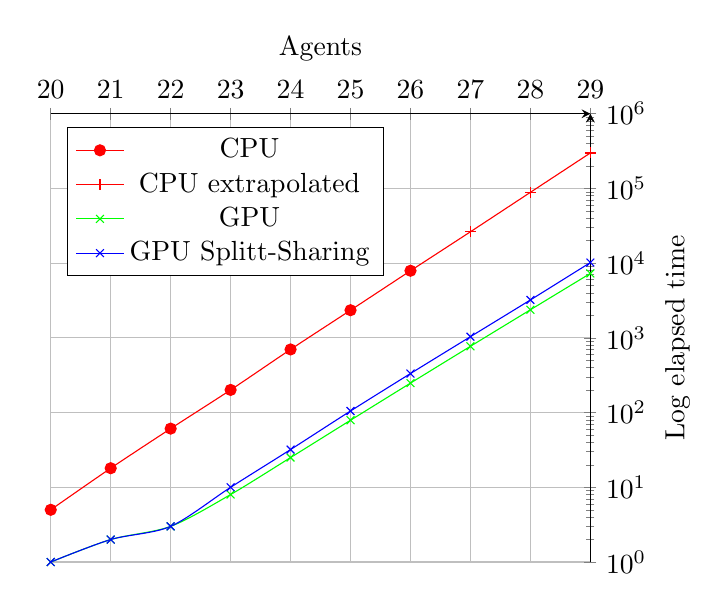
\begin{tikzpicture}[align=left]
\begin{axis}[
  xmin = 20,
  xmax = 29,
  ymax = 10e5,
  grid,
  xlabel={Agents},
  ylabel={Log elapsed time},
  xtick={20,...,29},
  axis lines=right, 
  legend pos= north west,
  ymode=log
    ]
\addplot[ mark = *,red,smooth] coordinates  
{( 20, 5 )
 ( 21, 18 )
 ( 22, 61 )
 ( 23, 201 )
 ( 24, 700 )
 ( 25, 2344 )
 ( 26, 7910 )
 }; 
 \addplot[ mark = +,red,smooth] coordinates  
{
 ( 26, 7910 )
 ( 27, 26302 )
 ( 28, 88644)
 ( 29, 298267)
 }; 
 
 \addplot[ mark = x,green,smooth] coordinates  
{( 20, 1 )
 ( 21, 2 )
 ( 22, 3 )
 ( 23, 8 )
 ( 24, 25 )
 ( 25, 79 )
 ( 26, 248 )
 ( 27, 771 )
 ( 28, 2376)
 ( 29, 7289)
 }; 

 \addplot[ mark = x,blue,smooth] coordinates  
{( 20, 1 )
 ( 21, 2 )
 ( 22, 3 )
 ( 23, 10 )
 ( 24, 32 )
 ( 25, 105 )
 ( 26, 333 )
 ( 27, 1037 )
 ( 28, 3218)
 ( 29, 10182)
 }; 

\legend{CPU,CPU extrapolated,GPU, GPU Splitt-Sharing}

\end{axis}
\end{tikzpicture}
\end{figure}
\section{Discussion} %not done
Figures \ref{nosplitt} and \ref{splitt} shows the difference between employing 
shared splittings discussed in section \ref{sectionsplit}. 
What it show are the number of logarithmic clock cycles elapsed between the 
previoius checkpoint and the current one as outline in algorithm \ref{dpgpu}.
What can first be noted is that checkpoint 4 is where the algorithm spends most of the time. 
Checkpoint 4 denote the generation of splittings and fetching them.
As mentioned earlier the algorithm is bandwidth bound and spending almost
$60\%$ of the time fetching memory shows that. Another reason of the result
is due to the not aligned random access making the effective bandwidth low.
Knowing that and looking at figure \ref{splitt} showing the result of sharing splittings it can be concluded that whilst it still spends most 
of the time fetching memory, henceforth improving the sharing of splittings make a significant impact on the overal performance.

Figure \ref{time} shows the difference between the CPU and GPU algorithm.
For every N agents the y axis shows the logarithmic elapsed time. The difference shown here between the implementations is substantial showing
that solving the problem on the GPU is highly beneficial. For 29 agents it solves it in 2 hours while the CPU bound algorithm was etrapolated to show that it would take up to 83 hours to complete. This is an speed factor of over 40 which would grow over the amount of agents. The reason it would grow is due to the implementations not being linearly parallel in logarithmic time where the GPU implementation having a smaller growth.
The difference between the GPU implementations where one utilizes internal 
sharing of splittings may also be noted to being $40\%$ faster than the variant without.
\section{Conclusion}
This paper show using the GPU to solve to Complete coalition structure formation problem is much viable option. 
Being so much faster it shows that

\section{Further work}
The notion of removing reduntant fetches from memory can be expanded into fully constructing the coalitions bottom up,
% \subsection{Math Equations}
% % You may want to display math equations in three distinct styles:
% % inline, numbered or non-numbered display.  Each of
% % the three are discussed in the next sections.
% 
% \subsubsection{Inline (In-text) Equations}
% A formula that appears in the running text is called an
% inline or in-text formula.  It is produced by the
% \textbf{math} environment, which can be
% invoked with the usual \texttt{{\char'134}begin. . .{\char'134}end}
% construction or with the short form \texttt{\$. . .\$}. You
% can use any of the symbols and structures,
% from $\alpha$ to $\omega$, available in
% \LaTeX\cite{Lamport:LaTeX}; this section will simply show a
% few examples of in-text equations in context. Notice how
% this equation: \begin{math}\lim_{n\rightarrow \infty}x=0\end{math},
% set here in in-line math style, looks slightly different when
% set in display style.  (See next section).

% \subsubsection{Display Equations}
% A numbered display equation -- one set off by vertical space
% from the text and centered horizontally -- is produced
% by the \textbf{equation} environment. An unnumbered display
% equation is produced by the \textbf{displaymath} environment.
% 
% Again, in either environment, you can use any of the symbols
% and structures available in \LaTeX; this section will just
% give a couple of examples of display equations in context.
% First, consider the equation, shown as an inline equation above:
% \begin{equation}\lim_{n\rightarrow \infty}x=0\end{equation}
% Notice how it is formatted somewhat differently in
% the \textbf{displaymath}
% environment.  Now, we'll enter an unnumbered equation:
% \begin{displaymath}\sum_{i=0}^{\infty} x + 1\end{displaymath}
% and follow it with another numbered equation:
% \begin{equation}\sum_{i=0}^{\infty}x_i=\int_{0}^{\pi+2} f\end{equation}
% just to demonstrate \LaTeX's able handling of numbering.
% 
% \subsection{Citations}
% Citations to articles \cite{bowman:reasoning,
% clark:pct, braams:babel, herlihy:methodology},
% conference proceedings \cite{clark:pct} or
% books \cite{salas:calculus, Lamport:LaTeX} listed
% in the Bibliography section of your
% article will occur throughout the text of your article.
% You should use BibTeX to automatically produce this bibliography;
% you simply need to insert one of several citation commands with
% a key of the item cited in the proper location in
% the \texttt{.tex} file \cite{Lamport:LaTeX}.
% The key is a short reference you invent to uniquely
% identify each work; in this sample document, the key is
% the first author's surname and a
% word from the title.  This identifying key is included
% with each item in the \texttt{.bib} file for your article.
% 
% The details of the construction of the \texttt{.bib} file
% are beyond the scope of this sample document, but more
% information can be found in the \textit{Author's Guide},
% and exhaustive details in the \textit{\LaTeX\ User's
% Guide}\cite{Lamport:LaTeX}.
% 
% This article shows only the plainest form
% of the citation command, using \texttt{{\char'134}cite}.
% This is what is stipulated in the SIGS style specifications.
% No other citation format is endorsed or supported.

% \subsection{Tables}
% Because tables cannot be split across pages, the best
% placement for them is typically the top of the page
% nearest their initial cite.  To
% ensure this proper ``floating'' placement of tables, use the
% environment \textbf{table} to enclose the table's contents and
% the table caption.  The contents of the table itself must go
% in the \textbf{tabular} environment, to
% be aligned properly in rows and columns, with the desired
% horizontal and vertical rules.  Again, detailed instructions
% on \textbf{tabular} material
% is found in the \textit{\LaTeX\ User's Guide}.
% 
% Immediately following this sentence is the point at which
% Table 1 is included in the input file; compare the
% placement of the table here with the table in the printed
% dvi output of this document.
% 
% \begin{table}
% \centering
% \caption{Frequency of Special Characters}
% \begin{tabular}{|c|c|l|} \hline
% Non-English or Math&Frequency&Comments\\ \hline
% \O & 1 in 1,000& For Swedish names\\ \hline
% $\pi$ & 1 in 5& Common in math\\ \hline
% \$ & 4 in 5 & Used in business\\ \hline
% $\Psi^2_1$ & 1 in 40,000& Unexplained usage\\
% \hline\end{tabular}
% \end{table}
% 
% To set a wider table, which takes up the whole width of
% the page's live area, use the environment
% \textbf{table*} to enclose the table's contents and
% the table caption.  As with a single-column table, this wide
% table will ``float" to a location deemed more desirable.
% Immediately following this sentence is the point at which
% Table 2 is included in the input file; again, it is
% instructive to compare the placement of the
% table here with the table in the printed dvi
% output of this document.
% 
% 
% \begin{table*}
% \centering
% \caption{Some Typical Commands}
% \begin{tabular}{|c|c|l|} \hline
% Command&A Number&Comments\\ \hline
% \texttt{{\char'134}alignauthor} & 100& Author alignment\\ \hline
% \texttt{{\char'134}numberofauthors}& 200& Author enumeration\\ \hline
% \texttt{{\char'134}table}& 300 & For tables\\ \hline
% \texttt{{\char'134}table*}& 400& For wider tables\\ \hline\end{tabular}
% \end{table*}
% % end the environment with {table*}, NOTE not {table}!
% 
% \subsection{Figures}
% Like tables, figures cannot be split across pages; the
% best placement for them
% is typically the top or the bottom of the page nearest
% their initial cite.  To ensure this proper ``floating'' placement
% of figures, use the environment
% \textbf{figure} to enclose the figure and its caption.
% 
% This sample document contains examples of \textbf{.ps}, \textbf{.eps} and \textbf{.pdf} files to be displayable with \LaTeX. Note that if you are using \textbf{pdflatex} to typeset your paper, you may only include \textbf{.pdf}, \textbf{.png}, \textbf{.jpeg} and \textbf{.gif} files in your paper. If, instead, you choose to use \textbf{latex} and \textbf{dvipdf} to typeset your paper, you may only include \textbf{.ps}, \textbf{.eps} files. More details on each of these is found in the \textit{Author's Guide}.
% 
% \begin{figure}
% \centering
% %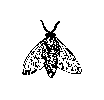
\includegraphics{fly.eps}
% \caption{A sample black and white graphic.}
% \end{figure}
% 
% \begin{figure}
% \centering
% %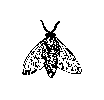
\includegraphics[width=height=1in, width=1in]{fly}
% \caption{A sample black and white graphic that has been resized with the \texttt{{\char'134}includegraphics} command.}
% \end{figure}
% 
% 
% As was the case with tables, you may want a figure
% that spans two columns.  To do this, and still to
% ensure proper ``floating'' placement of tables, use the environment
% \textbf{figure*} to enclose the figure and its caption.
% \begin{figure*}
% \centering
% %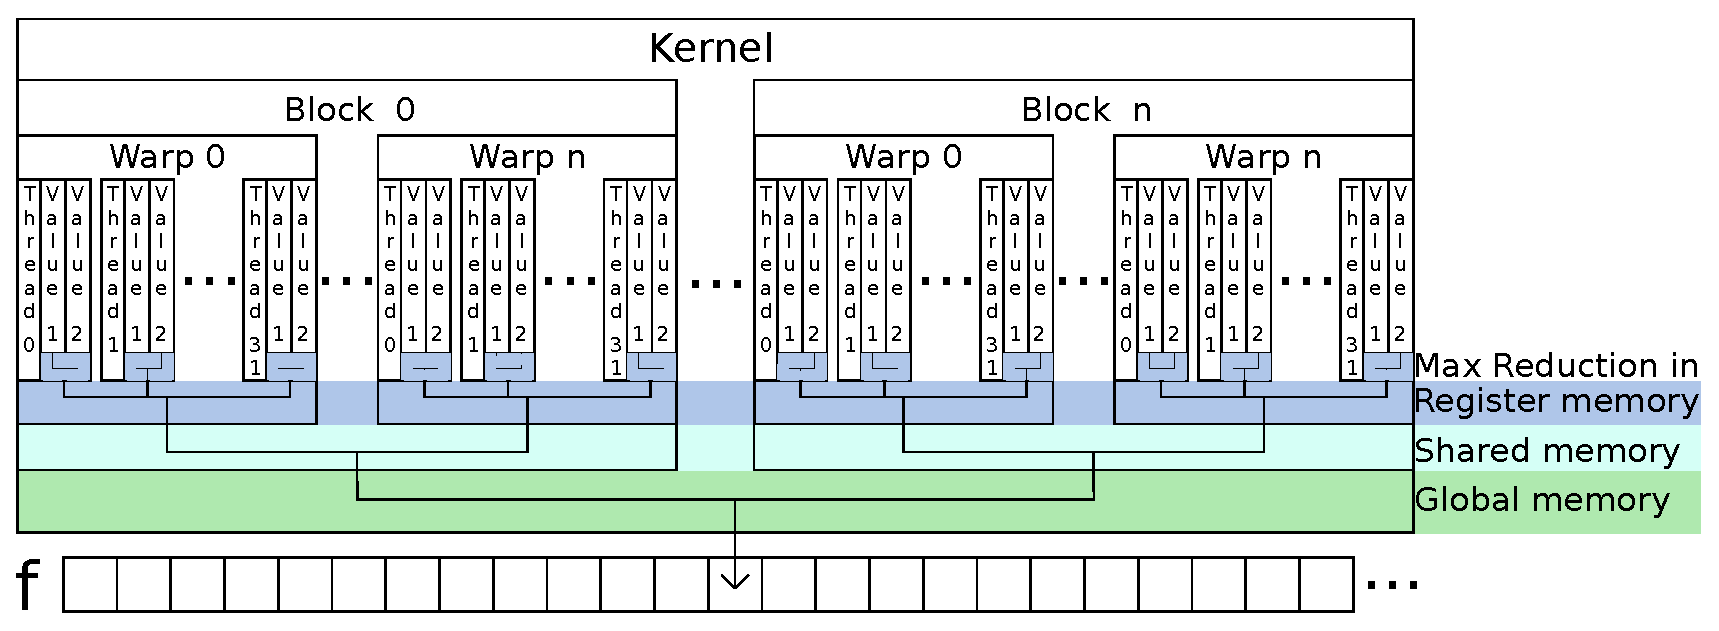
\includegraphics{reduction}
% \caption{A sample black and white graphic
% that needs to span two columns of text.}
% \end{figure*}
% and don't forget to end the environment with
% {figure*}, not {figure}!
% 
% %Note that either {\textbf{.ps}} or {\textbf{.eps}} formats are
% %used; use
% %the \texttt{{\char'134}epsfig} or \texttt{{\char'134}psfig}
% %commands as appropriate for the different file types.
% 
% \begin{figure}
% \centering
% %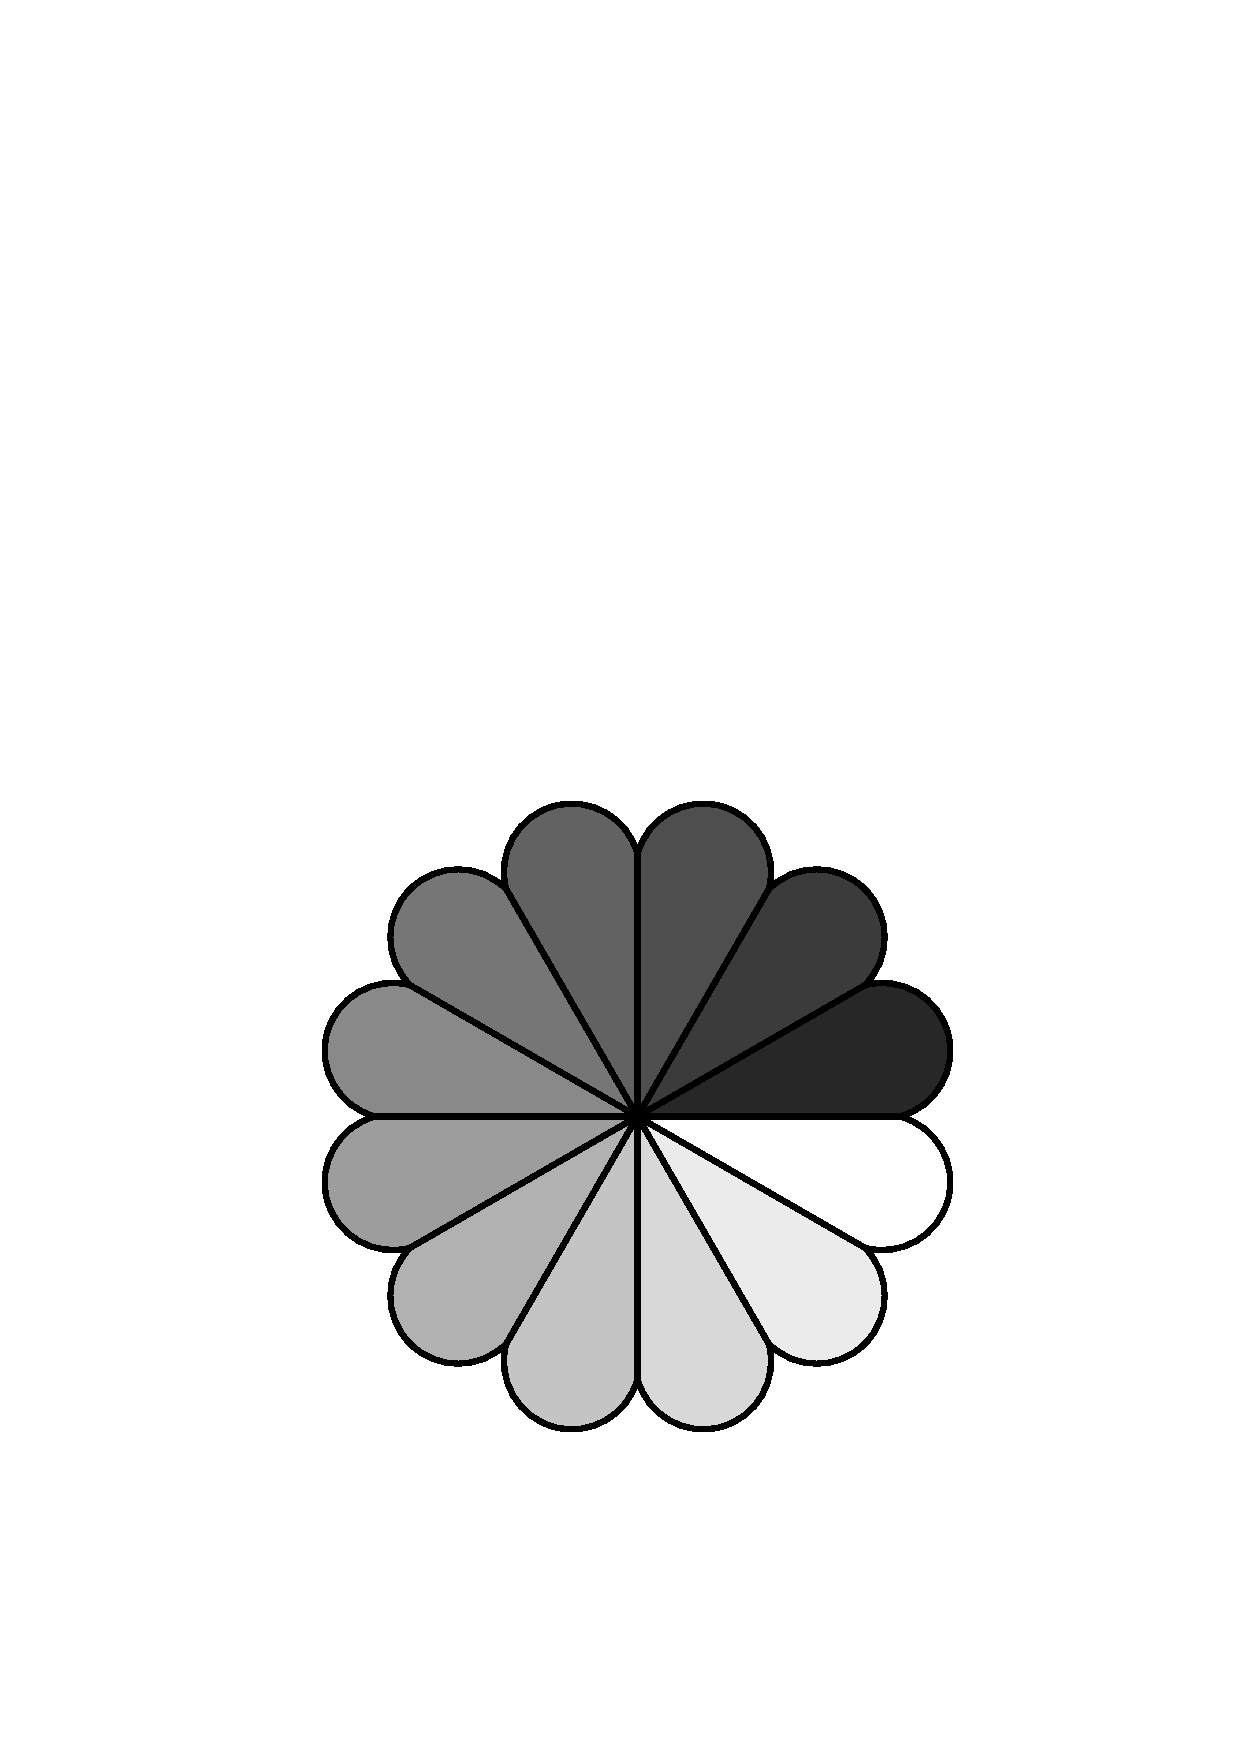
\includegraphics[width=\linewidth]{rosette}
% \caption{A sample black and white graphic that has
% been resized with the \texttt{{\char'134}includegraphics} command.}
% %\vskip -6pt
% \end{figure}
% 
% \subsection{Theorem-like Constructs}
% Other common constructs that may occur in your article are
% the forms for logical constructs like theorems, axioms,
% corollaries and proofs.  There are
% two forms, one produced by the
% command \texttt{{\char'134}newtheorem} and the
% other by the command \texttt{{\char'134}newdef}; perhaps
% the clearest and easiest way to distinguish them is
% to compare the two in the output of this sample document:
% 
% This uses the \textbf{theorem} environment, created by
% the\linebreak\texttt{{\char'134}newtheorem} command:
% \newtheorem{theorem}{Theorem}
% \begin{theorem}
% Let $f$ be continuous on $[a,b]$.  If $G$ is
% an antiderivative for $f$ on $[a,b]$, then
% \begin{displaymath}\int^b_af(t)dt = G(b) - G(a).\end{displaymath}
% \end{theorem}
% 
% The other uses the \textbf{definition} environment, created
% by the \texttt{{\char'134}newdef} command:
% \newdef{definition}{Definition}
% \begin{definition}
% If $z$ is irrational, then by $e^z$ we mean the
% unique number which has
% logarithm $z$: \begin{displaymath}{\log e^z = z}\end{displaymath}
% \end{definition}
% 
% Two lists of constructs that use one of these
% forms is given in the
% \textit{Author's  Guidelines}.
% 
% There is one other similar construct environment, which is
% already set up
% for you; i.e. you must \textit{not} use
% a \texttt{{\char'134}newdef} command to
% create it: the \textbf{proof} environment.  Here
% is a example of its use:
% \begin{proof}
% Suppose on the contrary there exists a real number $L$ such that
% \begin{displaymath}
% \lim_{x\rightarrow\infty} \frac{f(x)}{g(x)} = L.
% \end{displaymath}
% Then
% \begin{displaymath}
% l=\lim_{x\rightarrow c} f(x)
% = \lim_{x\rightarrow c}
% \left[ g{x} \cdot \frac{f(x)}{g(x)} \right ]
% = \lim_{x\rightarrow c} g(x) \cdot \lim_{x\rightarrow c}
% \frac{f(x)}{g(x)} = 0\cdot L = 0,
% \end{displaymath}
% which contradicts our assumption that $l\neq 0$.
% \end{proof}
% 
% Complete rules about using these environments and using the
% two different creation commands are in the
% \textit{Author's Guide}; please consult it for more
% detailed instructions.  If you need to use another construct,
% not listed therein, which you want to have the same
% formatting as the Theorem
% or the Definition\cite{salas:calculus} shown above,
% use the \texttt{{\char'134}newtheorem} or the
% \texttt{{\char'134}newdef} command,
% respectively, to create it.
% 
% \subsection*{A {\secit Caveat} for the \TeX\ Expert}
% Because you have just been given permission to
% use the \texttt{{\char'134}newdef} command to create a
% new form, you might think you can
% use \TeX's \texttt{{\char'134}def} to create a
% new command: \textit{Please refrain from doing this!}
% Remember that your \LaTeX\ source code is primarily intended
% to create camera-ready copy, but may be converted
% to other forms -- e.g. HTML. If you inadvertently omit
% some or all of the \texttt{{\char'134}def}s recompilation will
% be, to say the least, problematic.
% 
% \section{Conclusions}
% This paragraph will end the body of this sample document.
% Remember that you might still have Acknowledgments or
% Appendices; brief samples of these
% follow.  There is still the Bibliography to deal with; and
% we will make a disclaimer about that here: with the exception
% of the reference to the \LaTeX\ book, the citations in
% this paper are to articles which have nothing to
% do with the present subject and are used as
% examples only.
% %\end{document}
% 
% %ACKNOWLEDGMENTS are optional
% \section{Acknowledgments}
% This section is optional; it is a location for you
% to acknowledge grants, funding, editing assistance and
% what have you.  In the present case, for example, the
% authors would like to thank Gerald Murray of ACM for
% his help in codifying this \textit{Author's Guide}
% and the \textbf{.cls} and \textbf{.tex} files that it describes.

%
% The following two commands are all you need in the
% initial runs of your .tex file to
% produce the bibliography for the citations in your paper.
\bibliographystyle{abbrv}
\bibliography{sigproc}  % sigproc.bib is the name of the Bibliography in this case
% You must have a proper ".bib" file
%  and remember to run:
% latex bibtex latex latex
% to resolve all references
%
% ACM needs 'a single self-contained file'!
%
%APPENDICES are optional
%\balancecolumns
% \appendix
% %Appendix A
% \section{Headings in Appendices}
% The rules about hierarchical headings discussed above for
% the body of the article are different in the appendices.
% In the \textbf{appendix} environment, the command
% \textbf{section} is used to
% indicate the start of each Appendix, with alphabetic order
% designation (i.e. the first is A, the second B, etc.) and
% a title (if you include one).  So, if you need
% hierarchical structure
% \textit{within} an Appendix, start with \textbf{subsection} as the
% highest level. Here is an outline of the body of this
% document in Appendix-appropriate form:
% \subsection{Introduction}
% \subsection{The Body of the Paper}
% \subsubsection{Type Changes and  Special Characters}
% \subsubsection{Math Equations}
% \paragraph{Inline (In-text) Equations}
% \paragraph{Display Equations}
% \subsubsection{Citations}
% \subsubsection{Tables}
% \subsubsection{Figures}
% \subsubsection{Theorem-like Constructs}
% \subsubsection*{A Caveat for the \TeX\ Expert}
% \subsection{Conclusions}
% \subsection{Acknowledgments}
% \subsection{Additional Authors}
% This section is inserted by \LaTeX; you do not insert it.
% You just add the names and information in the
% \texttt{{\char'134}additionalauthors} command at the start
% of the document.
% \subsection{References}
% Generated by bibtex from your ~.bib file.  Run latex,
% then bibtex, then latex twice (to resolve references)
% to create the ~.bbl file.  Insert that ~.bbl file into
% the .tex source file and comment out
% the command \texttt{{\char'134}thebibliography}.
% % This next section command marks the start of
% % Appendix B, and does not continue the present hierarchy
% \section{More Help for the Hardy}
% The aamas2012 .cls file is based on the
% sig-alternate.cls file that is itself chock-full of succinct and
% helpful comments.  If you consider yourself a moderately experienced
% to expert user of \LaTeX, you may find reading it useful but please
% remember not to change it.
%\balancecolumns % GM June 2007
% That's all folks!
\end{document}
